\chapter{Theoretical Fundamentals} % Chapter title

\label{chapter:theoretical_fundamentals} % For referencing the chapter elsewhere, use \ref{chapter:computational_neuro} 

\def \blochwidth {0.4}
\def \qspherewidth {0.5}
\def \histogramwidth {0.4}
\newcommand{\bloch}{\emph{Bloch}-Sphere}
\newcommand{\qsphere}{Q-Sphere}
\newcommand{\hgate}{$\mathrm{H}$-Gate}

\newcommand{\xgate}{$\mathrm{X}$-Gate}
\newcommand{\ygate}{$\mathrm{Y}$-Gate}
\newcommand{\zgate}{$\mathrm{Z}$-Gate}

\newcommand{\rygate}{$\mathrm{RY}$-Gate}
\newcommand{\rxgate}{$\mathrm{RX}$-Gate}
\newcommand{\rzgate}{$\mathrm{RZ}$-Gate}

\newcommand{\crygate}{$\mathrm{CRY}$-Gate}
\newcommand{\crxgate}{$\mathrm{CRX}$-Gate}
\newcommand{\crzgate}{$\mathrm{CRZ}$-Gate}

\newcommand{\cxgate}{$\mathrm{CX}$-Gate}
\newcommand{\cygate}{$\mathrm{CY}$-Gate}
\newcommand{\czgate}{$\mathrm{CZ}$-Gate}

\newcommand{\frenchquotes}[1]{«~#1~»}

%----------------------------------------------------------------------------------------
\section{Quantum Computing}
Classical computing consist of 1s and 0s and has for years shaped the computational world and progress. Quantum computing is, from afar, similar. There are \emph{qubits}, which are comparable to classical \emph{bits}, but are fundamentally different. Whereas a bit can only have the state 0 or 1, a qubit allows the usage of any state, be it 0, 1 or a mix of those. Such a mix is referred to as a \emph{superposition}\cite{gudder_superposition_1970}. The catch comes when one wants to read the value of the qubit: one cannot directly measure its state, as visualized in figure \ref{figure:comparison_bit_qubit_measurement}.

\begin{figure}[!h]
    \centering
    \tikzset{every picture/.style={line width=0.75pt}} %set default line width to 0.75pt        
    
    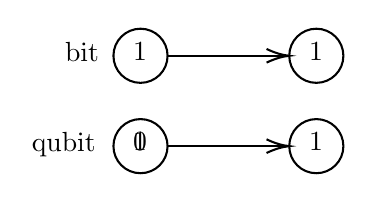
\begin{tikzpicture}[x=0.75pt,y=0.75pt,yscale=-1,xscale=1]
    %uncomment if require: \path (0,300); %set diagram left start at 0, and has height of 300
    % Text Node
    \draw    (117.29, 130) circle [x radius= 13.04, y radius= 13.04]   ;
    \draw (112.29,122) node [anchor=north west][inner sep=0.75pt]   [align=left] {1};
    % Text Node
    \draw    (202, 130) circle [x radius= 13.04, y radius= 13.04]   ;
    \draw (197,122) node [anchor=north west][inner sep=0.75pt]   [align=left] {1};
    % Text Node
    \draw    (202, 173.54) circle [x radius= 13.04, y radius= 13.04]   ;
    \draw (197,165.54) node [anchor=north west][inner sep=0.75pt]   [align=left] {1};
    % Text Node
    \draw (112.29,165.54) node [anchor=north west][inner sep=0.75pt]   [align=left] {0};
    % Text Node
    \draw    (117.29, 173.54) circle [x radius= 13.04, y radius= 13.04]   ;
    \draw (112.29,165.54) node [anchor=north west][inner sep=0.75pt]   [align=left] {1};
    % Text Node
    \draw (79.43,122) node [anchor=north west][inner sep=0.75pt]   [align=left] {bit};
    % Text Node
    \draw (63.43,165.54) node [anchor=north west][inner sep=0.75pt]   [align=left] {qubit};
    % Connection
    \draw    (130.32,173.54) -- (186.96,173.54) ;
    \draw [shift={(188.96,173.54)}, rotate = 180] [color={rgb, 255:red, 0; green, 0; blue, 0 }  ][line width=0.75]    (10.93,-3.29) .. controls (6.95,-1.4) and (3.31,-0.3) .. (0,0) .. controls (3.31,0.3) and (6.95,1.4) .. (10.93,3.29)   ;
    % Connection
    \draw    (130.32,130) -- (186.96,130) ;
    \draw [shift={(188.96,130)}, rotate = 180] [color={rgb, 255:red, 0; green, 0; blue, 0 }  ][line width=0.75]    (10.93,-3.29) .. controls (6.95,-1.4) and (3.31,-0.3) .. (0,0) .. controls (3.31,0.3) and (6.95,1.4) .. (10.93,3.29)   ;
    
    \end{tikzpicture}
    \caption{A comparison of measuring a single bit and a qubit. When measuring the bit, we get the same value that the bit is set to. When measuring a qubit, there is a certain probability of it being 0 and 1, so we measure one of both but don't know the real, internal state of the qubit.}
    \label{figure:comparison_bit_qubit_measurement}
\end{figure}

When measuring a quantum circuit, the qubit state collapses from a superposition into the fixed state of 0 or 1. This means that to measure the circuit an additional time, it has to be set up again. After doing multiple measurements on a qubit and collecting the results as shown in table \ref{table:example_counts}, the data can be used to construct a \emph{histogram}\cite{eckstein_lexikon_1994} akin to the one visualized in figure \ref{figure:example_histogram}, out of which one can retrieve the internal state of the qubit, which directly resembles the probabilities of measuring a 1 or 0 in the given circuit. The sum of these probabilities, be it per qubit or for a whole circuit, always amount to 1.

\begin{figure}[!h]
    \begin{subtable}{.5\textwidth}
    \centering
    \begin{tabular}{|c|c|}
         Measured value & Amount  \\
         \hline
         0 & 547 \\
         1 & 987 \\
    \end{tabular}
    \caption{Table containing all measurements done on a qubit in an unknown superposition. The number of occurrences of a measured 1 or 0 is counted and then used to generate the histogram in figure \ref{figure:example_histogram}}
    \label{table:example_counts}
    \end{subtable}
    \begin{subfigure}{.5\textwidth}
        \centering
        \scalebox{\histogramwidth}{
            \includesvg{thesis/Appendices/example_histogram.svg}
        }
        \caption{A histogram generated from the data in table \ref{table:example_counts}, that visually shows the probabilities of measuring 0 and 1. These probabilities can directly be used to understand the superposition of a qubit at the point of measurement.}
        \label{figure:example_histogram}
    \end{subfigure}
    \caption{Example of collected measurements from measuring an arbitrary single qubit in an unknown state, as well as the corresponding histogram generated from said data.}
    \label{fig:my_label}
\end{figure}

To further understand how a qubit behaves, the very foundations of quantum physics have to be looked at. Postulated by E. Schrödinger in 1925, the \emph{Schrödinger-Equation}\cite{PhysRev.28.1049} gives us the differential equation for the time evolution of a quantum state and their respective solution, shown in equation \ref{equation:schroedinger_time_evolution}, where $H$ denotes a Hamiltonian.

\begin{equation}
    \centering
    \begin{split}
          i\hbar\frac{d}{dt}\psi(t) =\ H\psi(t) \\
        \psi(t) =\ e^{-i\frac{Ht}{\hbar}}\psi(0)
    \end{split}
    \label{equation:schroedinger_time_evolution}
\end{equation}

The expression $U(t) =\ e^-i\frac{Ht}{\hbar}$ itself has the attribute that it is unitary. Through this, the multiplication of $U(t)$ with its conjugate transpose $U(t)^\ast$ results in the identity matrix. This leads to quantum operations being reversible – so-called \emph{bijective functions} - where every output can be reversed to a single input. \par
A mere two years later, Wolfgang Pauli published "Zur Quantenmechanik des magnetischen Elektrons"\cite{pauli_zur_1927}, in which he introduced the \emph{Pauli matrices}. These matrices represent the \emph{spin} of atoms and elementary particles, and are a core element of quantum computing. The definition of these matrices is shown in equation \ref{equation:pauli_matrices}.

\begin{equation}
    \centering
    \begin{split}
        \sigma_x &=\ \begin{pmatrix}0 & 1 \\ 1 & 0\end{pmatrix} =\ \mathrm{X}\\
        \sigma_y &=\ \begin{pmatrix}0 & -i \\ i & 0\end{pmatrix} =\ \mathrm{Y}\\
        \sigma_z &=\ \begin{pmatrix}1 & 0 \\ 0 & -1\end{pmatrix} =\ \mathrm{Z}\\
    \end{split}
    \label{equation:pauli_matrices}
\end{equation}

\newpage

The \bloch\cite{michael_a_nielsen_quantum_2000}, as shown in figure \ref{figure:basic_bloch_sphere}, is used to help visualize quantum operations on a single, \emph{non-entangled}, qubit. The complex \emph{Bloch}-Vector inside the \bloch\ (shown as pink arrow in figure \ref{figure:basic_bloch_sphere}) corresponds to the expectation value of measuring a certain value, 0 or 1, in a single qubit. To visualize entangled qubits, the \bloch\ by itself is not enough. There are proposed solutions to this problem\cite{gamel_entangled_2016}, which result in a more complex visualization with multiple \bloch s. To somewhat solve this issue in a simpler fashion, IBM's python library \code{qiskit} offers the Q-Sphere\cite{ibm_quantum_visualizations_nodate} as shown in figure \ref{figure:q_sphere_4qubit_h}, which can visualize up to 5 entangled single qubits. In addition, it can also show the probability of a given state through the diameter of the pointer next to a state, as shown in figure \ref{figure:q_sphere_4qubit_h}. Whilst the Q-Sphere also shows the phase of each state, it is not further used in this thesis.

\begin{figure}[!h]
    \centering
    \begin{subfigure}{.4\textwidth}
        \centering
        \scalebox{.6}{
            \includesvg{thesis/Appendices/Bloch_Sphere_axis.svg}
        }
        \caption{A basic \bloch\ with a visualized \emph{Bloch}-Vector, shown as the pink arrow. The axis $x$ and $y$ are annotated accordingly, but the axis $z$ is annotated with $\ket{0}$ and $\ket{1}$ - the states which are measured and have a corresponding probability assigned to them.}
        \label{figure:basic_bloch_sphere}
    \end{subfigure}
    \begin{subfigure}{.4\textwidth}
        \centering
        \scalebox{\qspherewidth}{
            \includesvg{thesis/Appendices/Q_Sphere_State_h_multiqubit.svg}
        }
        \caption{A basic Q-Sphere that shows all possible states of a 4 qubit circuit, as well as the probability of each state and their phase. The probability is encoded into the width of the pointers next to the state labels. As all pointers are equal, it is clear that all states have the same probability of being measured.}
        \label{figure:q_sphere_4qubit_h}
    \end{subfigure}
    \caption{A comparison of the \bloch\ used to visualize single qubits only, and the Q-Sphere that can visualize up to 5 qubits.}
    \label{fig:comparison_bloch_sphere_q_sphere}
\end{figure}

\newpage

When measuring a qubit, the state collapses onto the $z$-axis\cite{feynman_feynman_1965}, which in turn leads to a measurement of either 0 or 1. As a qubit can be in an arbitrary state of $\ket{0}$, $\ket{1}$ or anything in between, the state, also referred to as state-vector, of a single qubit is best described as  $\alpha\ket{0}+\beta\ket{1}$, whereas $|\alpha|^2 + |\beta|^2 = 1$\cite{qiskit_representing_nodate}. This directly describes the given amplitude of the measurable states a qubit can be in.\par
Quantum circuits generated using \code{qiskit} have all qubits initially set to state $\ket{0}$, which is visualized onto the Q-Sphere in figure \ref{figure:state_0_q_sphere}. This leads to the description of the qubits state being $1\ket{0}+0\ket{1}$, so it can be shortened to $\ket{0}$. A circuit that results in said state is visualized in figure \ref{figure:state_0_circuit}, and its mathematical counterpart in equation \ref{equation:state_0_equation}. The states $\ket{\psi_i}$ are used throughout the thesis to denote the state of one, or multiple, qubits at the currently marked point of the circuit.

\begin{figure}[!h]
    \begin{subfigure}{.5\textwidth}
    \centering
        \scalebox{\qspherewidth}{
            \includesvg{thesis/Appendices/Q_Sphere_State_0.svg}
        }
        \caption{A Q-Sphere with the state $\ket{0}$ visualized onto it.}
        \label{figure:state_0_q_sphere}
    \end{subfigure}
    \begin{subfigure}{.5\textwidth}
    \centering
        \scalebox{1.0}{
        \Qcircuit @C=1.0em @R=1.0em @!R { \\
    	 	\nghost{{q} :  } & \lstick{{q} :  } \barrier[0em]{0} & \qw & \qw & \qw\\
    	 	\nghost{} & \lstick{} & \ket{\psi_0} &\\
    \\ }}
        \caption{A basic circuit consisting of a single qubit $q$ that is initially set to $\ket{0}$. The state vector at point $\ket{\psi_0}$ is shown in equation \ref{equation:state_0_equation}.}
        \label{figure:state_0_circuit}
    \end{subfigure}
    \caption{A single qubit circuit with qubit state $\ket{0}$ at position $\ket{\psi_0}$ and its corresponding Q-Sphere visualization.}
    \label{fig:showcase_qubit_state_0_with_circuit}
\end{figure}



\begin{equation}
    \centering
    \begin{split}
        \ket{\psi_0} =\ \begin{pmatrix}1 \\ 0\end{pmatrix} =\ \ket{0}\\
    \end{split}
    \label{equation:state_0_equation}
\end{equation}

\newpage

To create the state $\ket{1}$, the circuit from figure \ref{figure:state_0_circuit} is extended with the Pauli \xgate\cite{qiskit_xgate_nodate}. The \xgate\ is the quantum equivalent to the classical NOT-Gate, which itself is an inverter and converts the state 0 to 1 and vice versa. To verify the behaviour of the \xgate, equation \ref{equation:state_1_equation} takes the state \xgate\ and multiplies the state $\ket{\psi_0}$ with it, which then results in the state $\ket{\psi_1}$, as noted on the circuit \ref{figure:x_circuit}, whilst the figure \ref{figure:state_1_q_sphere} visualizes the final state $\ket{\psi_1}$ on the Q-Sphere.

\begin{figure}[!h]
    \begin{subfigure}{.5\textwidth}
        \centering
        \scalebox{\blochwidth}{
            \includesvg{thesis/Appendices/Q_Sphere_State_1.svg}
        }
        \caption{The Q-Sphere with the state $\ket{\psi_1} =\ \ket{1}$ visualized onto it, which is achieved through the usage of the circuit in figure \ref{figure:x_circuit} and calculated in equation \ref{equation:state_1_equation}.}
        \label{figure:state_1_q_sphere}
    \end{subfigure}
    \begin{subfigure}{.5\textwidth}
        \centering\scalebox{1.0}{
        \Qcircuit @C=1.0em @R=0.2em @!R { \\
    	 	\nghost{{q} :  } & \lstick{{q} :  } \barrier[0em]{0} & \qw & \gate{\mathrm{X}} \barrier[0em]{0} & \qw & \qw & \qw\\
    	 	\nghost{} & \lstick{} & \ket{\psi_0} & & \ket{\psi_1} &\\
    \\ }}
        \caption{The circuit from figure \ref{figure:state_0_circuit} extended with a \xgate\ to transform the initial state $\ket{0}$ at position $\ket{\psi_0}$, into the state $\ket{1}$ at position $\ket{\psi_1}$, as calculated in equation \ref{equation:state_1_equation}.}
        \label{figure:x_circuit}
    \end{subfigure}
    \caption{A single qubit circuit with a \xgate\, where the single qubit has state $\ket{1}$ at position $\ket{\psi_1}$ and its corresponding Q-Sphere visualization.}
    \label{fig:showcase_qubit_state_1_with_circuit}
\end{figure}

\begin{equation}
    \centering
    \begin{split}
        \ket{\psi_1} =\ \mathrm{X}\ket{\psi_0} =\ \begin{pmatrix} 0 & 1\\ 1 & 0\end{pmatrix}\begin{pmatrix}1 \\ 0\end{pmatrix} =\ \begin{pmatrix}0 \\ 1 \end{pmatrix}\\
    \end{split}
    \label{equation:state_1_equation}
\end{equation}

As shown in equation \ref{equation:pauli_matrices}, there exist two more Pauli matrices. Like the \xgate\ that corresponds to the Pauli matrix $\sigma_x$, the gates \ygate\cite{qiskit_ygate_nodate} and \zgate\cite{qiskit_zgate_nodate} correspond to the Pauli matrices $\sigma_y$ and $\sigma_z$. \par

\newpage
It is important to note that depending on the state of a qubit, certain gates might not lead to a change in the probabilities of measuring a certain outcome. As shown in figure \ref{figure:showcase_z_gate}, the \zgate\ by itself does not change the possible outcome of a basic circuit, as calculated in equation \ref{equation:state_z_equation}.

\begin{figure}[!h]
    \begin{subfigure}{.5\textwidth}
        \centering
        \scalebox{\blochwidth}{
            \includesvg{thesis/Appendices/Q_Sphere_State_z.svg}
        }
        \caption{The Q-Sphere with the state $\ket{\psi_1} =\ \ket{0}$ visualized onto it, which is achieved through the usage of the circuit in figure \ref{figure:z_circuit} and calculated in equation \ref{equation:state_z_equation}.}
        \label{figure:state_z_sphere}
    \end{subfigure}
    \begin{subfigure}{.5\textwidth}
        \centering\scalebox{1.0}{
        \Qcircuit @C=1.0em @R=0.2em @!R { \\
    	 	\nghost{{q} :  } & \lstick{{q} :  } \barrier[0em]{0} & \qw & \gate{\mathrm{Z}} \barrier[0em]{0} & \qw & \qw & \qw\\
    	 	\nghost{} & \lstick{} & \ket{\psi_0} & & \ket{\psi_1} &\\
    \\ }}
        \caption{The circuit from figure \ref{figure:state_0_circuit} extended with a \zgate\ to transform the initial state $\ket{0}$ at position $\ket{\psi_0}$. As calculated in equation \ref{equation:state_z_equation}, the \zgate\ by itself does not change the possible measured state.}
        \label{figure:z_circuit}
    \end{subfigure}
    \caption{A single qubit circuit with a \zgate, where the single qubit has state $\ket{0}$ at position $\ket{\psi_1}$ and its corresponding Q-Sphere visualization.}
    \label{figure:showcase_z_gate}
\end{figure}

\begin{equation}
    \centering
    \begin{split}
        \ket{\psi_1} =\ \mathrm{Z}\ket{\psi_0} =\ \begin{pmatrix} 1 & 0\\ 0 & -1\end{pmatrix}\begin{pmatrix}1 \\ 0\end{pmatrix} =\ \begin{pmatrix}1 \\ 0\end{pmatrix}\\
    \end{split}
    \label{equation:state_z_equation}
\end{equation}

To achieve an equal probability of measuring the states $\ket{0}$ and $\ket{1}$, the \emph{Hadamard}-Gate, or \hgate\cite{qiskit_hgate_nodate}, can be used to change the state of a qubit from $\ket{0}$ to $\frac{1}{\sqrt{2}}\ket{0} + \frac{1}{\sqrt{2}}\ket{1}$ in one step. Without it, one would have to use a combination of different gates to achieve the result\cite{voorhoede_hadamard_nodate}, for example $\mathrm{XY}^{\frac{1}{2}}$. Figure \ref{figure:_one_qubit_h_state_circuit_qsphere} shows a circuit with the \hgate\ as well as the Q-Sphere for it. Equation \ref{equation:equal_superposition_equation} shows the calculation of the state $\ket{\phi_1}$ after the \hgate.


\begin{figure}[!h]
    \begin{subfigure}{.5\textwidth}
        \centering
        \scalebox{\blochwidth}{
            \includesvg{thesis/Appendices/Q_Sphere_State_h.svg}
        }
        \caption{A basic \qsphere\ with the state $\frac{1}{\sqrt{2}}\left(\ket{0} + \ket{1}\right)$ visualized onto it. The equal probability of both states is visualized through the blue dots, which have the same size.}
        \label{figure:state_h_q_sphere}
    \end{subfigure}
    \begin{subfigure}{.5\textwidth}
        \centering\scalebox{1.0}{
        \Qcircuit @C=1.0em @R=0.2em @!R { \\
    	 	\nghost{{q} :  } & \lstick{{q} :  } \barrier[0em]{0} & \qw & \gate{\mathrm{H}} \barrier[0em]{0} & \qw & \qw & \qw\\
    	 	\nghost{} & \lstick{} & \ket{\psi_0} & & \ket{\psi_1} &\\
    \\ }}
        \caption{A simple circuit with one qubit, that is transformed
    through the usage of a \hgate\ to turn the initial state $\ket{0}$ at position $\ket{\psi_0}$ into the state $\ket{1}$ at position $\ket{\psi_1}$. The calculation is shown in equation \ref{equation:equal_superposition_equation}.}
        \label{figure:h_circuit}
    \end{subfigure}
    \caption{A single qubit is set into an equal superposition shown on the \qsphere\ \ref{figure:state_h_q_sphere} generated using the circuit \ref{figure:h_circuit}}
    \label{figure:_one_qubit_h_state_circuit_qsphere}
\end{figure}



\begin{equation}
    \centering
    \begin{split}
        \ket{\psi_1} =\ \mathrm{H}\ket{\psi_0} =\ \frac{1}{\sqrt{2}}\begin{pmatrix} 1 & 1 \\ 1 & -1 \end{pmatrix}\begin{pmatrix}1 \\ 0\end{pmatrix} =\ \frac{1}{\sqrt{2}}\begin{pmatrix}1 \\ 0 \end{pmatrix} + \frac{1}{\sqrt{2}}\begin{pmatrix}0 \\ 1 \end{pmatrix}\\
    \end{split}
    \label{equation:equal_superposition_equation}
\end{equation}


To assess that the visualization in figure \ref{figure:state_h_q_sphere} and the described behaviour of the qubit is correct, these assumptions are evaluated formally by directly calculating the probability of measuring a given state. When calculating this probability, the Hermitian Transposition\cite{marshall_c_methods_1964} is used which results in the expression $p(\ket{x}) =\ |\bra{x}\ket{\psi}|^2$, with $\ket{\psi}$ being an arbitrary state of a quantum circuit. Equation \ref{equation:basic_h_measurement} demonstrates the calculation of the probabilities the \hgate\ assigns to the measurements of $0$ and $1$, using the state $\ket{\psi_1}$ from circuit \ref{figure:h_circuit}\cite{qiskit_representing_nodate}.

\begin{equation}[!h]
    \centering
    \begin{split}
        \ket{\psi_1} &=\ \frac{1}{\sqrt{2}}\ket{0} + \frac{1}{\sqrt{2}}\ket{1}\\
        \bra{0}\ket{\psi_1} &=\ \frac{1}{\sqrt{2}}\begin{pmatrix}1 & 0 \end{pmatrix}\begin{pmatrix}1 \\ 0 \end{pmatrix} + \frac{1}{\sqrt{2}}\begin{pmatrix}1 & 0 \end{pmatrix}\begin{pmatrix}0 \\ 1 \end{pmatrix} \\
        \bra{0}\ket{\psi_1} &=\ \frac{1}{\sqrt{2}}\\
        |\bra{0}\ket{\psi_1}|^2 &=\ 0.5\\
        |\bra{1}\ket{\psi_1}|^2 &=\ \left|\frac{1}{\sqrt{2}}\right|^2 =\ 0.5\\
    \end{split}
    \label{equation:basic_h_measurement}
\end{equation}

When desiring probabilities that are not equal for both states, the Pauli gates can be extended to support arbitrary parameters, which result in the gates \rygate\cite{qiskit_rygate_nodate}, \rxgate\cite{qiskit_rxgate_nodate} and \rzgate\cite{qiskit_rzgate_nodate}. These allow a parameter to be supplied, and therefore, change the probabilities. To create a circuit that achieves the probabilities from the histogram \ref{figure:example_histogram}, one can use the parameterized \rygate. To understand how these gates came to be, the equation \ref{equation:ry_gate_proof} shows how the findings in equations \ref{equation:schroedinger_time_evolution} and \ref{equation:pauli_matrices} are used to create the \rygate. The same can be done for the \rxgate\ and \rzgate. Note that the resulting power series in equation \ref{equation:ry_gate_proof} is the same as the power series for $\cos$ and $\sin$ shown in equation \ref{equation:power_series_sin_cos}\cite{lars_complex_1978}.

\begin{equation}
    \centering
    \begin{split}
        \mathrm{RY}(\theta) &=\ e^{-i\frac{\theta}{2}\mathrm{Y}} =\ e^{\frac{-i\theta}{2}\begin{pmatrix} 0 & -i \\ i & 0 \end{pmatrix}} \\
        \mathrm{Y}' &=\ -i\frac{\theta}{2}\mathrm{Y} =\ \begin{pmatrix}
                                                         0 & \frac{-\theta}{2}\\
                                                         \frac{\theta}{2} & 0\\
                                                    \end{pmatrix} \\
        e^{\mathrm{Y}'} &=\ I^{2\times2} + \mathrm{Y}' + \frac{\mathrm{Y}'^2}{2!} + \frac{\mathrm{Y}'^3}{3!} + \frac{\mathrm{Y}'^4}{4!} + \cdot\cdot\cdot \\
        \mathrm{RY}(\theta) &=\ \begin{pmatrix}
         1 - \frac{\theta^2}{8} + \frac{\theta^4}{384} + \cdot\cdot\cdot & - \frac{\theta}{2} + \frac{\theta^3}{48} - \frac{\theta^5}{3840} + \cdot\cdot\cdot\\
         \frac{\theta}{2} - \frac{\theta^3}{48} + \frac{\theta^5}{3840} + \cdot\cdot\cdot & 1 - \frac{\theta^2}{8} + \frac{\theta^4}{384} + \cdot\cdot\cdot \\
         \end{pmatrix}\\ &=\ \begin{pmatrix}
        \cos{\frac{\theta}{2}} & -\sin{\frac{\theta}{2}} \\
        \sin{\frac{\theta}{2}} & \cos{\frac{\theta}{2}}
    \end{pmatrix}
    \end{split}
    \label{equation:ry_gate_proof}
\end{equation}



\begin{equation}
    \begin{split}
        \cos(x) &=\ 1 - \frac{x^2}{2!} + \frac{x^4}{4!} - \frac{x^6}{6!} + \cdot\cdot\cdot \\
        \sin(x) &= x - \frac{x^3}{3!} + \frac{x^5}{5!} - \frac{x^7}{7!} + \cdot\cdot\cdot
    \end{split}
    \label{equation:power_series_sin_cos}
\end{equation}

The formal definition used in equation \ref{equation:basic_h_measurement} can be reversed and used with the \rygate\ to calculate the parameters needed to achieve the probabilities shown in \ref{figure:example_histogram}, as shown in equation \ref{equation:parameter_from_probabilities}. 

\begin{equation}
    \centering
    \begin{split}
        |\bra{1}\ket{\psi_1}|^2 &=\ 0.643 \\
        \begin{pmatrix}0 & 1\end{pmatrix}\ket{\psi_1} &=\ \sqrt{0.643} \\
        \begin{pmatrix}1 & 0\end{pmatrix}\ket{\psi_1} &=\ \sqrt{0.357} \\
        \ket{\psi_1} &=\ \sqrt{0.357}\begin{pmatrix} 1 \\ 0\end{pmatrix} + \sqrt{0.643}\begin{pmatrix} 0 \\ 1\end{pmatrix}\\
        \ket{\psi_1} &=\ \begin{pmatrix}\sqrt{0.357}\\ \sqrt{0.643}\end{pmatrix}\\
        \mathrm{RY}(\theta)\ket{0} &=\ \begin{pmatrix}\sqrt{0.357}\\ \sqrt{0.643}\end{pmatrix} \\
        \begin{pmatrix}\cos{\frac{\theta}{2}} \\ -i\sin{\frac{\theta}{2}}\end{pmatrix} &=\ \begin{pmatrix}\sqrt{0.357}\\ \sqrt{0.643}\end{pmatrix}\\
        \theta_{cos} &=\ 2(\acos{\sqrt{0.357}}) =\ 1.8608\\
        \theta_{sin} &=\ 2(\asin{\sqrt{0.643}}) =\ 1.8608\\
        \theta &=\ \theta_{sin} =\ \theta_{cos}\\
    \end{split}
    \label{equation:parameter_from_probabilities}
\end{equation}

With the value of $\theta$ calculated, the circuit \ref{figure:circuit_for_histogram} is designed and evaluated to compare it to the histogram from \ref{figure:example_histogram}, as shown in figure \ref{figure:circuit_histogram}. The programming language used is \code{Python} with IBM's library \code{qiskit}\cite{Qiskit}, that allows the creation of quantum circuits, as well as running and measuring them in either a simulator or real quantum hardware.


\begin{listing}[!h]
    \centering
    \begin{minted}{python}
    circuit = QuantumCircuit(1)
    circuit.ry(1.8608, 0)
    circuit.measure_all()
    backend = Aer.get_backend('qasm_simulator')
    job = backend.run(transpile(circuit, backend), shots=1024)
    result = job.result()
    counts=result.get_counts(circuit)
    plot_histogram(counts)
    \end{minted}
    \caption{\code{Python} code using \code{qiskit} to create the circuit represented in figure \ref{figure:circuit_for_histogram}, that is executed and results in the histogram \ref{figure:circuit_histogram}}
    \label{figure:code_circuit_histogram_for_example_data}
\end{listing}

\begin{figure}[!h]
    \begin{subfigure}{.5\textwidth}
        \centering
        \scalebox{\histogramwidth}{
            \includesvg{thesis/Appendices/calculated_circuit_histogram.svg}
        }
        \caption{A histogram, generated from the data in table \ref{table:example_counts}, that visually shows the probabilities of 0 and 1 of the qubit on the circuit \ref{figure:circuit_for_histogram}.}
        \label{figure:circuit_histogram}
    \end{subfigure}
    \begin{subfigure}{.5\textwidth}
        \centering
        \scalebox{1.0}{
        \Qcircuit @C=1.0em @R=0.2em @!R { \\
        	 	\nghost{{q} :  } & \lstick{{q} :  } & \gate{\mathrm{R_Y}\,(\mathrm{1.8608})} & \qw & \qw\\
        \\ }}
        \caption{A circuit designed with a parameterized \rygate using the code from figure \ref{figure:code_circuit_histogram_for_example_data}. The parameter is the one calculated in equation \ref{equation:parameter_from_probabilities} and generates the histogram \ref{figure:circuit_histogram}, which results in the same data as in the example histogram \ref{figure:example_histogram}.}
        \label{figure:circuit_for_histogram}
    \end{subfigure}
    \caption{A quantum circuit with a parameterized \rygate\ that is used to generate the histogram that resembles the one used as example in figure \ref{figure:example_histogram}}
    \label{figure:figure_circuit_histogram_rebuilt_from_example}
\end{figure}

\newpage

One critical part of quantum computing is the entanglement of multiple qubits. This entanglement dictates that the qubits enter a state where one cannot explain their isolated state, but has to express the state of the whole system as a sum of its parts. As previously noted, this is the reason why the \bloch\ cannot be used in entangled, multi-qubit circuits, as it can only correctly show the state of one non-entangled qubit. Schrödinger E. fully explained entanglement in 1935\cite{schroedinger_discussion_entanglement}, whereafter Einstein A. called it \emph{spukhafte Fernwirkung}, or \emph{spooky action at a distance}, as entangled particles enact upon each other at any distance – therefore breaking the speed of light defined in Einstein A.'s \emph{Theory of relativity}\cite{einstein_grundlage_1916}.  \par
In \code{qiskit}, entanglement of multiple qubits can be achieved through the usage of \emph{controlled} gates. These gates, in their simplest form, cross two qubits. One of those is the \emph{controlling} qubit, which dictates if the gate is applied on the \emph{target} qubit or not. The most simple gates, built again using the \emph{Pauli matrices}, are the CX-Gate\cite{qiskit_cxgate_nodate}, CY-Gate\cite{qiskit_cygate_nodate} and CZ-Gate\cite{qiskit_czgate_nodate}. Circuit \ref{circuit:example_h_cx_circuit} shows a two qubit circuit with an CX-Gate applied onto both qubits, using $q_0$ as \emph{controlling} qubit and $q_1$ as \emph{target} qubit. Equation \ref{equation:cx_construction} shows the mathematical construction of the CX-Gate, where $q_0$ is the control qubit and $q_1$ is the target qubit. The CX-Gate behaves like a classical NOT gate – therefore, negating the value of the target – with an additional input to turn it \emph{on} or \emph{off}.

\begin{equation}
    \centering
    \begin{split}
    CX\ q_0, q_1 &=
    I \otimes |0\rangle\langle0| + X \otimes |1\rangle\langle1| \\
    &= \begin{pmatrix}1 & 0\\0 & 1\end{pmatrix}\otimes\begin{pmatrix}1 & 0 \\ 0 & 0\end{pmatrix} + \begin{pmatrix}0 & 1\\1 & 0\end{pmatrix}\otimes\begin{pmatrix}0 & 0 \\ 0 & 1\end{pmatrix} \\
    &= \begin{pmatrix}
        1 & 0 & 0 & 0 \\
        0 & 0 & 0 & 1 \\
        0 & 0 & 1 & 0 \\
        0 & 1 & 0 & 0
    \end{pmatrix}
    \end{split}
    \label{equation:cx_construction}
\end{equation}

As shown in equation \ref{equation:cx_construction}, the CX matrix is of size $4\times4$. This is larger than the dimension of the state of a single qubit, due to the fact of it applying to two qubits at once. When applying such a gate, one has to merge both states of the used qubits to create a state vector with increased dimensionality. This is done by calculating the tensor product of both qubits, as shown in equation \ref{equation:example_tensor_product}, and the resulting state vector can be directly compared to a vector containing all possible states one can measure. As $q0$ has the state $\ket{0}$ and $q_1$ the state $\ket{1}$, the only possible outcome to a measurement would be the $10$\footnote{This means the result is formatted as Little-Endian, with the first bit being the rightmost one, in this case $q_1q_0$.}.

\begin{equation}
    \centering
    \begin{split}
        \ket{0} \otimes \ket{1} =\ \begin{pmatrix}1 \\ 0\end{pmatrix} &\otimes \begin{pmatrix}0 \\ 1\end{pmatrix} =\ \begin{pmatrix} 0 \\ 0 \\ 1 \\ 0 \end{pmatrix} \\
        \begin{pmatrix} 0 \\ 0 \\ 1 \\ 0 \end{pmatrix} &\rightarrow \begin{pmatrix}00 \\ 01 \\ 10 \\ 11\end{pmatrix}
    \end{split}
    \label{equation:example_tensor_product}
\end{equation}

Figure \ref{circuit:example_h_cx_circuit} contains a single \hgate\ that is applied on $q_0$, as well as a \cxgate\ applied on $q_0$ and $q_1$. Equation \ref{equation:states_cx_circuit} calculates the resulting probabilities at $\ket{\psi_1}$ and shows that there is a chance of measuring $00$ or $11$. As $q_0$ has the H-Gate applied, it sits at an equal superposition and has the same probability of measuring 0 or 1. In the case of $q_0$ being 1, the CX-Gate activates and flips the value of $q_1$, which is up until that point $\ket{0}$. This leads to the only possible, measurable states being $00$ and $11$.


\begin{figure}[!h]
    \centering
    \scalebox{1.0}{
\Qcircuit @C=1.0em @R=0.2em @!R { \\
	 	\nghost{{q}_{0} :  } & \lstick{{q}_{0} :  } & \gate{\mathrm{H}} \barrier[0em]{1} & \qw & \ctrl{1} \barrier[0em]{1} & \qw & \qw & \qw\\
	 	\nghost{{q}_{1} :  } & \lstick{{q}_{1} :  } & \qw & \qw & \targ & \qw & \qw & \qw\\
	 	\nghost{} & \lstick{} &  &  \ket{\psi_0} &  & \ket{\psi_1} & \\
\\ }}
    \caption{Simple two qubit circuit where the \hgate\ is applied to $q_0$ and afterwards both qubits $q_0$ and $q_1$ are entangled using a CX-Gate. The states $\ket{\psi_0}$ and $\ket{\psi_1}$ symbolize the state of the system before and after the CX-Gate.}
    \label{circuit:example_h_cx_circuit}
\end{figure}

\begin{equation}
    \centering
    \begin{split}
    \ket{\psi_0}_{q_0} &=\ \frac{1}{\sqrt{2}}\ket{0} + \frac{1}{\sqrt{2}}\ket{1}\\
    \ket{\psi_0}_{q_1} &=\ \ket{0}\\
    \ket{\psi_1} &=\ \mathrm{CX}\ket{0}\otimes\begin{pmatrix}\frac{1}{\sqrt{2}} \\ \frac{1}{\sqrt{2}}\end{pmatrix} \\
    \ket{\psi_1} &=\ \begin{pmatrix}
    1 & 0 & 0 & 0\\
    0 & 0 & 0 & 1\\
    0 & 0 & 1 & 0\\
    0 & 1 & 0 & 0\\
    \end{pmatrix}\begin{pmatrix}\frac{1}{\sqrt{2}} \\ \frac{1}{\sqrt{2}} \\ 0 \\ 0\end{pmatrix} \\
    \ket{\psi_1} &=\ \begin{pmatrix}\frac{1}{\sqrt{2}} \\ 0 \\ 0 \\ \frac{1}{\sqrt{2}}\end{pmatrix} \rightarrow \begin{pmatrix}00 \\ 01 \\ 10 \\ 11\end{pmatrix}
    \end{split}
    \label{equation:states_cx_circuit}
\end{equation}


%%%%%%%%%%%%%%%%%%%%%%%%%%%%%%%%%%%%%%


\newpage

\section{Quantum Neural Network}
\label{chapter:qnn}

The \textit{classic computational neuron} originally proposed by Rosenblatt F.\cite{rosenblatt_perceptron_1958}, as shown in figure \ref{figure:classic_computational_neuron}, builds the basis for most classical neural networks used today. The underlying principle is simple and shown in equation \ref{equation:classical_neuron_computation}. All inputs $x_n$ are multiplied by a corresponding weight $w_n$, then their total sum calculated. The resulting value is passed to an activation function $f(x)$, which is activated if a predefined threshold value is exceeded. The activation function $f(x)$, also called transfer function, can be selected from a plethora of valid choices\cite{szandala_review_2021}.

\tikzset{every picture/.style={line width=0.75pt}} %set default line width to 0.75pt        
\begin{figure}[h!]
    \centering

    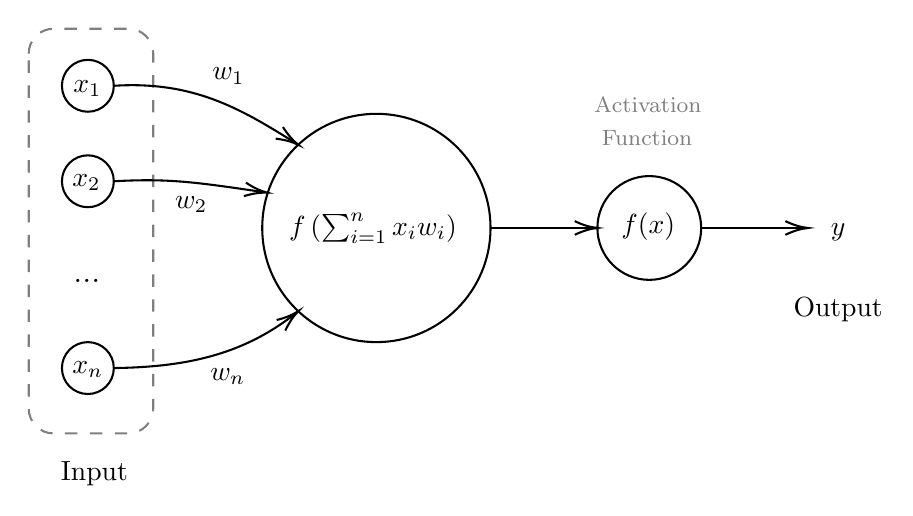
\begin{tikzpicture}[x=0.75pt,y=0.75pt,yscale=-1,xscale=1]
    %uncomment if require: \path (0,300); %set diagram left start at 0, and has height of 300
    
    %Shape: Circle [id:dp6859812572471455] 
    \draw   (192.5,140) .. controls (192.5,109.62) and (217.12,85) .. (247.5,85) .. controls (277.88,85) and (302.5,109.62) .. (302.5,140) .. controls (302.5,170.38) and (277.88,195) .. (247.5,195) .. controls (217.12,195) and (192.5,170.38) .. (192.5,140) -- cycle ;
    %Shape: Circle [id:dp24070647763127284] 
    \draw   (96,71.5) .. controls (96,64.6) and (101.6,59) .. (108.5,59) .. controls (115.4,59) and (121,64.6) .. (121,71.5) .. controls (121,78.4) and (115.4,84) .. (108.5,84) .. controls (101.6,84) and (96,78.4) .. (96,71.5) -- cycle ;
    %Shape: Circle [id:dp9363816782656273] 
    \draw   (96,117.5) .. controls (96,110.6) and (101.6,105) .. (108.5,105) .. controls (115.4,105) and (121,110.6) .. (121,117.5) .. controls (121,124.4) and (115.4,130) .. (108.5,130) .. controls (101.6,130) and (96,124.4) .. (96,117.5) -- cycle ;
    %Shape: Circle [id:dp4720861626805333] 
    \draw   (96,207.5) .. controls (96,200.6) and (101.6,195) .. (108.5,195) .. controls (115.4,195) and (121,200.6) .. (121,207.5) .. controls (121,214.4) and (115.4,220) .. (108.5,220) .. controls (101.6,220) and (96,214.4) .. (96,207.5) -- cycle ;
    %Rounded Rect [id:dp5631408345855224] 
    \draw  [color={rgb, 255:red, 0; green, 0; blue, 0 }  ,draw opacity=0.5 ][dash pattern={on 4.5pt off 4.5pt}] (80,56) .. controls (80,49.37) and (85.37,44) .. (92,44) -- (128,44) .. controls (134.63,44) and (140,49.37) .. (140,56) -- (140,227) .. controls (140,233.63) and (134.63,239) .. (128,239) -- (92,239) .. controls (85.37,239) and (80,233.63) .. (80,227) -- cycle ;
    %Curve Lines [id:da4059065253769214] 
    \draw    (121,71.5) .. controls (159.22,69.05) and (182.07,82.45) .. (208.38,98.98) ;
    \draw [shift={(210,100)}, rotate = 212.2] [color={rgb, 255:red, 0; green, 0; blue, 0 }  ][line width=0.75]    (10.93,-3.29) .. controls (6.95,-1.4) and (3.31,-0.3) .. (0,0) .. controls (3.31,0.3) and (6.95,1.4) .. (10.93,3.29)   ;
    %Curve Lines [id:da5094425475664381] 
    \draw    (121,207.5) .. controls (153.51,207.01) and (182.13,202.15) .. (208.78,180.98) ;
    \draw [shift={(210,180)}, rotate = 140.83] [color={rgb, 255:red, 0; green, 0; blue, 0 }  ][line width=0.75]    (10.93,-3.29) .. controls (6.95,-1.4) and (3.31,-0.3) .. (0,0) .. controls (3.31,0.3) and (6.95,1.4) .. (10.93,3.29)   ;
    %Curve Lines [id:da5523039314594727] 
    \draw    (121,117.5) .. controls (147.6,116.02) and (160.61,117.94) .. (193.48,122.78) ;
    \draw [shift={(195,123)}, rotate = 188.37] [color={rgb, 255:red, 0; green, 0; blue, 0 }  ][line width=0.75]    (10.93,-3.29) .. controls (6.95,-1.4) and (3.31,-0.3) .. (0,0) .. controls (3.31,0.3) and (6.95,1.4) .. (10.93,3.29)   ;
    %Straight Lines [id:da007343534667061169] 
    \draw    (302.5,140) -- (352,140) ;
    \draw [shift={(354,140)}, rotate = 180] [color={rgb, 255:red, 0; green, 0; blue, 0 }  ][line width=0.75]    (10.93,-3.29) .. controls (6.95,-1.4) and (3.31,-0.3) .. (0,0) .. controls (3.31,0.3) and (6.95,1.4) .. (10.93,3.29)   ;
    %Shape: Circle [id:dp683884067109112] 
    \draw   (354,140) .. controls (354,126.19) and (365.19,115) .. (379,115) .. controls (392.81,115) and (404,126.19) .. (404,140) .. controls (404,153.81) and (392.81,165) .. (379,165) .. controls (365.19,165) and (354,153.81) .. (354,140) -- cycle ;
    %Straight Lines [id:da9286309330170883] 
    \draw    (404,140) -- (453.5,140) ;
    \draw [shift={(455.5,140)}, rotate = 180] [color={rgb, 255:red, 0; green, 0; blue, 0 }  ][line width=0.75]    (10.93,-3.29) .. controls (6.95,-1.4) and (3.31,-0.3) .. (0,0) .. controls (3.31,0.3) and (6.95,1.4) .. (10.93,3.29)   ;
    
    % Text Node
    \draw (100,163) node [anchor=north west][inner sep=0.75pt]   [align=left] {{\large ...}};
    % Text Node
    \draw (100,67.4) node [anchor=north west][inner sep=0.75pt]    {$x_{1}$};
    % Text Node
    \draw (99.5,112.9) node [anchor=north west][inner sep=0.75pt]    {$x_{2}$};
    % Text Node
    \draw (99.5,202.9) node [anchor=north west][inner sep=0.75pt]    {$x_{n}$};
    % Text Node
    \draw (94,251) node [anchor=north west][inner sep=0.75pt]   [align=left] {Input};
    % Text Node
    \draw (167,61.4) node [anchor=north west][inner sep=0.75pt]    {$w_{1}$};
    % Text Node
    \draw (149,123.4) node [anchor=north west][inner sep=0.75pt]    {$w_{2}$};
    % Text Node
    \draw (166,206.4) node [anchor=north west][inner sep=0.75pt]    {$w_{n}$};
    % Text Node
    \draw (204,131.4) node [anchor=north west][inner sep=0.75pt]    {$f\left(\sum _{i=1}^{n} x_{i} w_{i} \right)$};
    % Text Node
    \draw (447,172) node [anchor=north west][inner sep=0.75pt]   [align=left] {Output};
    % Text Node
    \draw (364,131.4) node [anchor=north west][inner sep=0.75pt]    {$f( x)$};
    % Text Node
    \draw (465,136.4) node [anchor=north west][inner sep=0.75pt]    {$y$};
    % Text Node
    \draw (351,67) node [anchor=north west][inner sep=0.75pt]  [color={rgb, 255:red, 0; green, 0; blue, 0 }  ,opacity=0.5 ] [align=left] {\begin{minipage}[lt]{38.1pt}\setlength\topsep{0pt}
    \begin{center}
    {\footnotesize Activation}\\{\footnotesize Function}
    \end{center}
    
    \end{minipage}};
    
    \end{tikzpicture}

    \caption{Visual representation of the classic computational neuron, often referred to as a perceptron.}
    \label{figure:classic_computational_neuron}
\end{figure}

\begin{equation}
    \centering
    y =\ f\left(\sum_{i = 1}^n x_i\omega_i\right)
    \label{equation:classical_neuron_computation}
\end{equation}

Rosenblatt’s perceptron is basically a single-layer neural network and is limited in its capabilities. To overcome the practical limitations, we can use multiple perceptrons in a specific structure to build a so-called multilayer perceptron, as illustrated in figure \ref{figure:classic_multilayer_perceptron} \cite{haykin2009neural}.


\begin{figure}[h!]
    \centering
    \scalebox{0.8}{
        \begin{tikzpicture}[x=2.2cm,y=1.4cm]
          \readlist\Nnod{4,3,3,2} % array of number of nodes per layer
          \readlist\Nstr{n,m,m,m,k} % array of string number of nodes per layer
          \readlist\Cstr{\strut x,a^{(\prev)},a^{(\prev)},a^{(\prev)},y} % array of coefficient symbol per layer
          \def\yshift{0.5} % shift last node for dots
          
          \message{^^J  Layer}
          \foreachitem \N \in \Nnod{ % loop over layers
            \def\lay{\Ncnt} % alias of index of current layer
            \pgfmathsetmacro\prev{int(\Ncnt-1)} % number of previous layer
            \message{\lay,}
            \foreach \i [evaluate={\c=int(\i==\N); \y=\N/2-\i-\c*\yshift;
                         \index=(\i<\N?int(\i):"\Nstr[\lay]");
                         \x=\lay; \n=\nstyle;}] in {1,...,\N}{ % loop over nodes
              % NODES
              \node[node \n] (N\lay-\i) at (\x,\y) {$\Cstr[\lay]_{\index}$};
              
              % CONNECTIONS
              \ifnum\lay>1 % connect to previous layer
                \foreach \j in {1,...,\Nnod[\prev]}{ % loop over nodes in previous layer
                  \draw[connect,white,line width=1.2] (N\prev-\j) -- (N\lay-\i);
                  \draw[connect] (N\prev-\j) -- (N\lay-\i);
                  %\draw[connect] (N\prev-\j.0) -- (N\lay-\i.180); % connect to left
                }
              \fi % else: nothing to connect first layer
              
            }
            \path (N\lay-\N) --++ (0,1+\yshift) node[midway,scale=1.5] {$\vdots$};
          }
          
          % LABELS
          % \node[above=5,align=center,mygreen!60!black] at (N1-1.90) {input\\[-0.2em]layer};
          % \node[above=2,align=center,myblue!60!black] at (N3-1.90) {hidden layers};
          % \node[above=10,align=center,myred!60!black] at (N\Nnodlen-1.90) {output\\[-0.2em]layer};
          
        \end{tikzpicture}
    }
    \caption{Example illustration of a classical, multilayer perceptron, also referred to as artificial neural network. From left to right: Input layer in green, two hidden layers in blue and the output layer in red.}
    \label{figure:classic_multilayer_perceptron}
\end{figure}

\vspace{2em}
The quantum analogue of a classical neuron is called a quantum neuron, also referred to as \textit{quron}, as proposed by Maria Schuld et al.\cite{schuldQuestQuantumNeural2014a}. The classical perceptron cannot be implemented one-to-one as a \textit{quron} because of the nature of quantum computations. Thus, the strategy is to replicate the functionality of a classical perceptron using a quantum algorithm, built as a quantum circuit. These quantum circuits can vary in structure and gates use. Currently known implementations are the \textit{QFT-based perceptron}\cite{SchuldSimulatingAPerceptron_2015}, \textit{Repeat Until Success circuits}\cite{QuantumNeuronAnElementaryBuildingBlock,Torrontegui_2019} and \textit{Non-linearity from measurement}\cite{tacchinoArtificialNeuronImplemented2019}, among others\cite{AltaiskyQuantumNeuralNetwork,DesignOfQuantumNeuronModel}, and serve different computational use cases.\par
Just as a classical neural network can be built and extended in varying fashion, the same can be said about its quantum counterpart. There are differing interpretations and implementations of quantum neural networks\cite{Mangini_2021,Mitarai_2018,ClassificationWithQNN,QNNConceptsApplicationsChallenges,Killoran_2019}. It has yet to be shown what the best and most exact representation of a neural network as quantum circuit is. For example, one could represent the whole neural network as one quantum circuit, try to replace the perceptrons with a quantum analogue etc.\cite{OnQuantumNeuralNetworks,Ezhov2000,schuldQuestQuantumNeural2014a} Additionally, there are various approaches and different views on which classical part corresponds to which quantum analogue or if every step in a classical neural network could or even should have its quantum counterpart\cite{OnQuantumNeuralNetworks,Ezhov2000,schuldQuestQuantumNeural2014a}. \par
A different publication by Schuld et al.\cite{schuldCircuitcentricQuantumClassifiers2020} states that a quantum circuit closely resembles a neural network with unitary layers, whereas Abbas et al.\cite{Abbas_2021,schuldCircuitcentricQuantumClassifiers2020} states that quantum neural networks are a subclass of \textit{Variational Quantum Algorithms} or VQAs, consisting of quantum circuits with parameterised gates. Furthermore, VQAs with parameterised gates, also known as \textit{Variational Quantum Circuits} VQCs, are especially promising when running on current quantum hardware, also referred to as \textit{Noisy Intermediate-Scale Quantum} or NISQ. 

\subsection{Variational Quantum Algorithm (VQA)}
\label{subsection:vqa_fundamentals}
According to Cerezo et al.\cite{Cerezo_2021}, VQAs are a framework that consists of basic buildings blocks used to solve a variety of problems. These building blocks usually accommodate at least one kind of VQC, as shown in figure \ref{fig:general_scheme_vqc}. VQAs are arguably the quantum analogue of highly successful machine-learning methods, such as neural networks. Moreover, VQAs leverage the toolbox of classical optimization, since they use VQCs to run on a quantum computer, and outsource the parameter optimization to a classical optimizer. This method describes a hybrid classical-quantum algorithm with supervised learning.

\begin{figure}[!h]
    \centering
    \scalebox{0.8}{
		\Qcircuit @C=1.4em @R=.8em {
            \lstick{\ket{0}} & \multigate{3}{Feature\ Map} & \multigate{3}{Variational\ Model} & \meter \\
            \lstick{\ket{0}} & \ghost{Feature\ Map} & \ghost{Variational\ Model} & \meter \\
            \vdots           & \nghost{Feature\ Map} & \nghost{Variational\ Model} & \vdots \\
            \lstick{\ket{0}} & \ghost{Feature\ Map} & \ghost{Variational\ Model} & \meter \\
            & & & \\
	    }
    }
    \caption{General scheme of a \textit{variational quantum circuit}. The circuit is initialized as zero state $\ket{0}$, followed by the feature 
    embedding (see chapter \ref{subsection:quantum_embedding_using_a_feature_map}) then continued by a variational model which incorporates trainable parameters, finally ending with measurements on each qubit.} 
    \label{fig:general_scheme_vqc}
\end{figure}

\textbf{Hybrid classical-quantum algorithms} utilize both classical and quantum computers. Frankhauser et al.\cite{fankhauser_multiple_2021} state that these types of algorithms are considered promising since they can better handle erroneous, small-scale quantum devices than “pure” quantum algorithms. The algorithm performs the embedding of features and parameters, as well as the measurement of the circuit for the classification, as shown in figure \ref{fig:schematic_hybrid_classical_quantum}. The actual classification, parameter optimizations as well as loss and accuracy calculations are done using classical methods. 

\begin{figure}[!h]
    \centering
    \scalebox{0.88}{
        \begin{tikzpicture}[
          roundnode/.style={circle, draw=black!60, fill=white!5, thick, minimum size=7mm},
          squarednode/.style={rectangle, draw=black!60, fill=white!5, thick, minimum size=10mm},
          optimizernode/.style={rectangle, draw=black!60, fill=white!5, thick, minimum size=25mm},
          quantumcircuit/.style={draw=blue, minimum height=3.5cm, minimum width=10cm, fill=white!5, label=below:{\color{blue}variational quantum\ circuit}},
        ]
            %Nodes
            \node[roundnode]        (dataset)        {Data};
            \node[squarednode]      (preprocess)     [right=of dataset] {Preprocessing};
            \node                   (point1)         [below=of preprocess] {};
            \node[quantumcircuit]   (quantumcircuit) [below right=of dataset]  {
                \Qcircuit @C=1em @R=.7em {
                    \lstick{\ket{0}} & \multigate{3}{feature\ embedding} & \multigate{3}{model\ circuit} & \meter & \cw \\
                    \lstick{\ket{0}} & \ghost{feature\ embedding} & \ghost{model\ circuit} & \meter & \cw \\
                    \cdots & \nghost{feature\ embedding} & \nghost{model\ circuit} & \cdots &  \\
                    \lstick{\ket{0}} & \ghost{feature\ embedding} & \ghost{model\ circuit} & \meter & \cw \gategroup{1}{5}{4}{5}{1.5em}{\}}
                }
            };
            \node[optimizernode]      (optimizer)     [right=of quantumcircuit] {Optimizer};
            % Lines
            \draw[->] (dataset.east) -- (preprocess.west);
            \draw[->] (quantumcircuit.east) -- (optimizer.west);
            \draw [->] (preprocess.south) -- ++(0,-.6) -- ++(+1.3,0) -| ++(0,-0.6);
            \draw [->] (optimizer.north) -- ++(0,+1.25) -- ++(-6.15,0) node[auto,midway,above] {parameter updates} -| ++(0,-1);
        \end{tikzpicture}
    }
    \caption{Schematic view of the hybrid classical-quantum algorithm. Everything outside the \textit{variational quantum circuit} inside the blue box is done with classical methods.}
    \label{fig:schematic_hybrid_classical_quantum}
\end{figure}


As showcased in figure \ref{fig:schematic_hybrid_classical_quantum}, the data is loaded and preprocessed once at the beginning. It is then split into two subsets $D_{training}, D_{testing} \in D$, whereas $\forall x \in D_{training}, \forall y \in D_{testing} | x \notin D_{testing} \wedge y \noting D_{training}$. Afterwards, multiple training iterations are done with the following procedure:

\begin{enumerate}
    \item A variational quantum circuit is constructed by embedding the features from $D_{training}$ into the quantum state using a feature map. In addition, the optimized parameters are also embedded into the quantum state\footnote{During the first iteration, the parameters are chosen at random}.
    \item The created VQC is executed either on the simulator or real hardware and a result acquired.
    \item The acquired result is parsed and compared to the expected result.
    \item According to the result, the optimizer modifies the parameters and starts a new iteration.
\end{enumerate}

The algorithm stops if a certain threshold or the maximum iteration count for the optimization is reached. The trained parameters can now be embedded into a new quantum circuit and used to evaluate the testing subset $D_{testing}$.

\subsection{Quantum embedding using a Quantum Feature Map}
\label{subsection:quantum_embedding_using_a_feature_map}
Quantum embedding, -encoding and feature embedding, -encoding both refer to the same procedure, namely the representation of classical data in the Hilbert space by through the usage of a quantum feature map. 
More formally and corresponding to Havlicek et al.\cite{havlicekSupervisedLearningQuantum2019}, a quantum feature map is an injective encoding of classical information $\vec{x} \in \mathbb{R}^d$ into a quantum state $\op{\psi}{\psi}$ on a $n$-qubit register. Here, $\mathcal{H}_2 = \mathbb{C}^2$ is a Hilbert space consisting of a single qubit, and $\mathcal{S}(\mathcal{H}_2^{\otimes n})$ denotes the cone of positive semidefinite density matrices\footnote{Density matrices are explained in \cite{homeister2008quantum}.} $p \geq 0$ with unit trace $tr(p) = 1$. This cone is a subset of the $4^n$ dimensional Hilbert space of $\mathcal{M}_{2^n\times2^n}(\mathbb{C})$ (The reader is referred to Puchała et al.\cite{PuchałaStrategiesQuantumMeasurements} work for a detailed explanation). The feature map acts as seen in equation \ref{equation:feature_map_acts_as}

\begin{equation}
    \centering
    \begin{split}
        \Phi : \Omega \subset \mathbb{R}^d \rightarrow \mathcal{S}(\mathcal{H}_2^{\otimes n}), \qquad \Phi : \vec{x} \mapsto \op{\Phi(\vec{x})}{\Phi(\vec{x})}
    \end{split}
    \label{equation:feature_map_acts_as}
\end{equation}

The action of the map can be understood by a unitary circuit family denoted $\mathcal{U}_{\Phi(\vec{x})}$ that is applied to some reference state, i.e. $\ket{0}^n$. The resulting state is given by $\ket{\Phi(\vec{x})} = \mathcal{U}_{\Phi(\vec{x})}\ket{0}^n$. The state in the feature space should depend non-linearly on the data.\cite{havlicekSupervisedLearningQuantum2019,schuld_SQMLmodelsAreKernelMethods,SchuldEffectOfDataEncoding_2021}

\subsection{Kernel-Based Support Vector Machines and Quantum Support Vector Machines (QSVM)}
A classical support vector machine (SVM) also known as support vector network and initially proposed by Cortes et al.\cite{Cortes2004SupportVectorN}, divides a set of objects into classes in such a way that the widest possible area around the class boundaries remains free of objects. A detailed explanation on how classical support vector machines work can be found in the work of Fletcher et al.\cite{fletcher2009support}. Quantum SVMs is considered to be the quantum analogue of the classical SVMs algorithm as stated by Jiaying Yang et al.\cite{yangSupportVectorMachines2019}.\par
SVMs can not only perform linear classifications but also non-linear ones using the so-called kernel trick. Kernel-Based SVMs use a feature function $\phi(\vec{x})$ to map data points into a higher dimension with advantageous properties for classification, thus re-writing the linear decision function in terms of a dot product between data points. By combining this product with the feature function, we can substitute it with a kernel function as shown in equation \ref{equation:svm_kernel_function} with some feature space $\mathcal{H}$.\cite{ThomsenComparingQNNs_QSVM} 

\begin{equation}
    \centering
    \begin{split}
        k(\vec{x}, \vec{x}^{(i)}) = \expval{\phi(\vec{x}^{(i)}),\phi(\vec{x})}_{\mathcal{H}} 
    \end{split}
    \label{equation:svm_kernel_function}
\end{equation}

According to Thomsen et al.\cite{ThomsenComparingQNNs_QSVM}, using an already classified data point $\vec{x}^{(i)}$ and a to be classified data point $\vec{x}$, the corresponding decision function uses the kernel function to classify $\vec{x}$, as shown in equation \ref{equation:svm_alternative_decision_function}.

\begin{equation}
    \centering
    \begin{split}
        \tilde{c}_{SVM}(\vec{x})  &=\ sign\left(\sum_{i=1}^M a_i y_i \expval{\phi(\vec{x}^{(i)}),\phi(\vec{x})}_{\mathcal{H}} + b\right)
    \end{split}
    \label{equation:svm_alternative_decision_function}
\end{equation}

The quantum analogue kernel function equation – with an exponentially large space of density matrices $\mathcal{S}(2^q)$ spanned across $q$ qubits as the feature space – can be seen in equation \ref{equation:qsvm_kernel_function_preliminary}\cite{ThomsenComparingQNNs_QSVM}.

\begin{equation}
    \centering
    \begin{split}
        \psi: \mathbb{R}^S & \rightarrow \mathcal{S}(2^q)\\
        \vec{x} & \mapsto \op{\psi(\vec{x}^{(i)})}{\psi(\vec{x})}\\
        \rightarrow k(\vec{x}, \vec{x}^{(i)}) &= \left|\ip{\psi(\vec{x}^{(i)})}{\psi(\vec{x})}\right|^2
    \end{split}
    \label{equation:qsvm_kernel_function_preliminary}
\end{equation}

\subsection{Comparison QNN and QSVM}
\label{subsection:comparison_qnn_qsvm}
According to Havlicek et al.\cite{havlicekSupervisedLearningQuantum2019}, the generic decision function of an SVM classifier, as seen in equation \ref{equation:svm_decision_function}, has the same form as the decision function from a QNN seen in equation \ref{equation:qnn_decision_function}. Therefore, a QNN implements a linear decision boundary in a feature space. \textit{Note: The equations \ref{equation:svm_decision_function}, \ref{equation:qnn_decision_function}, \ref{equation:w_alpha_real_coefficient}, \ref{equation:psi_alpha_real_coefficient} and the descriptions between them have been taken from \cite{ThomsenComparingQNNs_QSVM}}.

\begin{equation}
    \centering
        \tilde{c}_{SVM}(\vec{x}) =\ sign\left(\ip{\Vec{w}}{\phi(\vec{x})}_{\mathcal{H}}+b\right)
    \label{equation:svm_decision_function}
\end{equation}

With $\vec{x}$ being input data in the original space $\mathbb{R}^s$, $\Vec{w} \in \mathcal{H}$, $\ip{\cdot}{\cdot}_{\mathcal{H}}$ being an inner product in $\mathcal{H}$ as well as $\mathcal{H}$ being a possibly infinite dimensional Hilbert space\footnote{A vector space with scalar product is called a Hilbert space if the property that every Cauchy sequence must converge is satisfied.}. Here, the notation $\Vec{w}$ is for vectors in the Hilbert/feature space. Bias is defined as $b \in [\-1, +1]$

\begin{equation}
    \centering
        \tilde{c}_{QNN}(\vec{x}) =\ sign\left(\frac{1}{2^q} \sum_{\alpha} w_{\alpha}(\theta)\psi_{\alpha}(\vec{x})+b\right)
    \label{equation:qnn_decision_function}
\end{equation}

$w_{\alpha}(\theta)$ and $\psi_{\alpha}(\vec{x})$ are the real coefficients and defined in equations \ref{equation:w_alpha_real_coefficient} and \ref{equation:psi_alpha_real_coefficient}.

\begin{equation}
    \centering
        w_{\alpha}(\theta) =\ tr\left(\mathcal{W}(\theta)^{\dag}\mathcal{F}\mathcal{W}(\theta)\mathcal{P}_{\alpha}\right)\footnotemark[1]
    \label{equation:w_alpha_real_coefficient}
\end{equation}

\begin{equation}
    \centering
        \psi_{\alpha}(\vec{x}) =\ tr\left(\op{\psi(\vec{x})}{\psi(\vec{x})}\mathcal{P}_{\alpha}\right)\footnotemark[1]
    \label{equation:psi_alpha_real_coefficient}
\end{equation}

\footnotetext[1]{We refer the reader to the papers \cite{havlicekSupervisedLearningQuantum2019,ThomsenComparingQNNs_QSVM} for the definition of $\mathcal{P}_{\alpha}$.}

The same is concluded by Schuld et al.\cite{schuld_SQMLmodelsAreKernelMethods} as seen in the illustration \ref{figure:2101.11020_Maria_Schuld_Fig.3} taken from their work, while stating: 

\begin{displayquote}
“The bridge between quantum machine learning and kernel methods is formed by the observation that quantum models map data into a high-dimensional feature space, in which the measurement defines a linear decision boundary.” — Schuld et al.\cite{schuld_SQMLmodelsAreKernelMethods}
\end{displayquote}

\begin{figure}[!h]
    \centering
    \includegraphics[width=0.7\linewidth]{thesis/Figures/qnn/2101.11020_Maria_Schuld_Fig.3.png} 
    \caption{Figure taken out of Schuld et al.\cite{schuld_SQMLmodelsAreKernelMethods} that shows how a given data space $\mathcal{X}$ is mapped to a feature space $\mathcal{M}$.}
    \label{figure:2101.11020_Maria_Schuld_Fig.3}
\end{figure}

\clearpage

While QNN and QSVM both implement a linear decision boundary in their respective feature spaces, the main difference lies in the variational circuit $\mathcal{W}(\theta)$, as shown in figure \ref{fig:general_structure_qsvm_and_qnn}.

\begin{figure}[!h]
    \centering
    \begin{subfigure}{1.0\textwidth}
        \centering
	    \scalebox{0.8}{
        \Qcircuit @C=1.4em @R=0.8em {
                & & \ket{\psi(\vec{x_i})} & & & \\
                & & & & & & \\
                \lstick{\ket{0}} & \multigate{3}{\qquad\mathcal{E}(\Vec{x_i})\qquad} \barrier[0em]{3} & \qw       & \multigate{3}{\qquad \mathcal{E}(\Vec{x_j})^{\dag} \qquad} & \meter \\
                \lstick{\ket{0}} & \ghost{\qquad\mathcal{E}(\Vec{x_i})\qquad}                         & \qw       & \ghost{\qquad \mathcal{E}(\Vec{x_j})^{\dag} \qquad}        & \meter \\
                \vdots           & \nghost{\qquad\mathcal{E}(\Vec{x_i})\qquad}                        & \nghost{} & \nghost{\qquad \mathcal{E}(\Vec{x_j})^{\dag} \qquad}       & \vdots \\
                \lstick{\ket{0}} & \ghost{\qquad\mathcal{E}(\Vec{x_i})\qquad}                         & \qw       & \ghost{\qquad \mathcal{E}(\Vec{x_j})^{\dag} \qquad}        & \meter \\
                & & & & & & \\
            }
    	}
    	\subcaption{General quantum circuit structure of a QSVM kernel estimator with a parametrized unitary $\mathcal{E}(\Vec{x_i})$ followed by its adjoint $\mathcal{E}(\Vec{x_j})^{\dag}$. The kernel can only be evaluated approximately with a finite number of measurement shots due to the probalistic nature of quantum computing.}
    	\label{subfigure:general_structure_qsvm}
    \end{subfigure}
    \\[2em]
    \begin{subfigure}{1.0\textwidth}
        \centering
	    \scalebox{0.8}{
        \Qcircuit @C=1.4em @R=0.8em {
                & & \ket{\psi(\vec{x})} & & & \\
                & & & & & & \\
                \lstick{\ket{0}} & \multigate{3}{\qquad\mathcal{U}_{\Phi(\Vec{x})}\qquad} \barrier[0em]{3} & \qw       & \multigate{3}{\qquad W(\theta) \qquad} & \meter \\
                \lstick{\ket{0}} & \ghost{\qquad\mathcal{U}_{\Phi(\Vec{x})}\qquad}                         & \qw       & \ghost{\qquad W(\theta) \qquad}        & \meter \\
                \vdots           & \nghost{\qquad\mathcal{U}_{\Phi(\Vec{x})}\qquad}                        & \nghost{} & \nghost{\qquad W(\theta) \qquad}       & \vdots \\
                \lstick{\ket{0}} & \ghost{\qquad\mathcal{U}_{\Phi(\Vec{x})}\qquad}                         & \qw       & \ghost{\qquad W(\theta) \qquad}        & \meter \\
                & & & & & & \\
            }
    	}
        \subcaption{General quantum circuit structure of a QNN, which is defined to consist of a feature map circuit $\mathcal{U}_{\Phi(\Vec{x})}$ followed by a variational form circuit $W(\theta)$ strictly separating the fixed input vector $\Vec{x}$ and trainable parameters $\theta$.}
    	\label{subfigure:general_structure_qnn}
    \end{subfigure}
    \caption{General schematics of a variational quantum circuit and quantum support vector machine circuit.}
    \label{fig:general_structure_qsvm_and_qnn}
\end{figure}

Thomsen further states the following: 

\begin{displayquote}
``The main difference between the QNN and QSVM now lies in the parameterized coefficients $w_{\alpha}(\theta)$ that make up the vector $w(\vec{\theta}) \in \mathcal{S}(\mathcal{H}_2^{\otimes n})$ that defines the direction of the hyperplane in feature space according to which class membership is assigned by the QNN. Because these coefficients are determined through a variational circuit $W(\theta)$, they can not take on arbitrary values in general. In particular, there is no guarantee that the solution to the dual QSVM optimization problem in (2.17) on page 12 denoted by $\vec{w}^*$ is accessible to the QNN. But $\vec{w}^*$ is guaranteed to be found by the QSVM due to convexity and guaranteed to maximize the (regularized by slack) margin in feature space by strong duality. With this, the QNN can be interpreted as an approximation to the QSVM that finds a solution that is at best equally good, depending on the expressivity of the variational form.'' — A. Thomsen\cite{ThomsenComparingQNNs_QSVM}\footnote[1]{The mentioned optimization problem equation 2.17 does not contain the denoted $\vec{w}^*$ which is a reference error and thus has been omitted in this thesis.}
\end{displayquote}

\clearpage

This can be compared to the findings of Schuld et al.\cite{schuld_SQMLmodelsAreKernelMethods} and their figure \ref{figure:2101.11020_Maria_Schuld_Fig.5}.

\begin{figure}[!h]
    \centering
    \includegraphics[width=1.0\textwidth]{thesis/Figures/qnn/2101.11020_Maria_Schuld_Fig.5.png} 
    \caption{Figure taken out of Schuld et al.\cite{schuld_SQMLmodelsAreKernelMethods}, that shows the differences in kernel-based training and variational training.}
    \label{figure:2101.11020_Maria_Schuld_Fig.5}
\end{figure}

Conclusively, the main difference between a QNN and a QSVM is the variational model, that is not guaranteed to find the optimal measurement and searches for it in a different subspace than the QSVM.
%%%%%%%%%%%%%%%%%%%%%%%%%%%%%%%%%%%%%%%%%%%%%%%

\newpage

\section{Multiple Query Optimization}
\label{chapter:fundamental_multiple_query_optimization}

A query\cite{codd_relational_1970} is a demand for information to be pulled from a database. Such a query can vary in size and structure, as well as in execution time. These are often written in the query language \code{SQL}, which is often adapted to the corresponding software\cite{shirgoldbird_microsoft_nodate}\cite{the_postgresql_global_development_group_postgresql_2022} it executes on. 

    
\begin{listing}[!ht]
    \centering
    \begin{minted}{sql}
        SELECT * FROM USERS u
        JOIN ADDRESSES
        ON ADDRESSES.UID = USERS.UID
        WHERE USERS.NAME = "Abraham"
    \end{minted}
    \caption{This example SQL code would tell the database we want to merge the content of the tables \code{USERS} and \code{ADDRESSES} together. The resulting table has rows for each user and their respective address. The data is also filtered, so that only the entries where the \code{NAME} is "Abraham" are inside the merged table.}
    \label{figure:sql_query_example}
\end{listing}

The example query in listing \ref{figure:sql_query_example} is parsed and results in one, or more, execution plans\cite{microsoft_execution_nodate}, always dependent on the query and the setup of the database. These plans are also referred to as query plans. The fastest plan then is selected and executed, which retrieves the desired data and displays it, as visualized in table \ref{table:sql_query_result_example}.

\begin{table}[!h]
    \centering
    \begin{tabular}{|c|c|c|c|c|c|c|}
        \hline
        Name    & Surname  & Address & Number & Zipcode & City & UID\\ \hline
        Abraham & Martin   & Neweg & 17b & 3249 & Nothingham & 43\\ \hline
        Abraham & Tart     & York & 95 & 12078 & Krypton & 34    \\ \hline
    \end{tabular}
    \caption{Exemplary data returned after executing the SQL query from figure \ref{figure:sql_query_example}, where the first row resembles the name of the attributes in the column}
    \label{table:sql_query_result_example}
\end{table}

To further understand the difference the execution brings, the assumption is made that table $A$ (for addresses) and $U$ (for users) both consist of 10'000 rows each.  Executing plan 1 would lead to the operation $M$ having to search and combine all 20'000 rows together, and then from the resulting 10'000 rows, select only those that fulfil the defined criteria. In plan 2, the table $U$ is filtered beforehand, which results in smaller number of rows, and hence, fewer rows to merge for the operation $M$. Whilst this might not lead to a particular speed up in this case, as soon as queries get more complex, and for example join more than two tables, the saved time start to add up.\par
The query in figure \ref{figure:sql_query_example} already allows for \emph{at least} two different query plans during execution. These are shown in figure \ref{figure:example_query_plans}. The nodes $U$ and $A$ stand for the operation of loading the tables \code{USERS} and \code{ADDRESSES} from the storage. The node $M$ stands for the merging of the tables, and the node $S$ for selecting the rows that fulfil the defined filter of \code{USER.NAME = "Abraham"}.

\begin{figure}[!h]
    \centering
    \tikzset{every picture/.style={line width=0.75pt}} %set default line width to 0.75pt        
    
    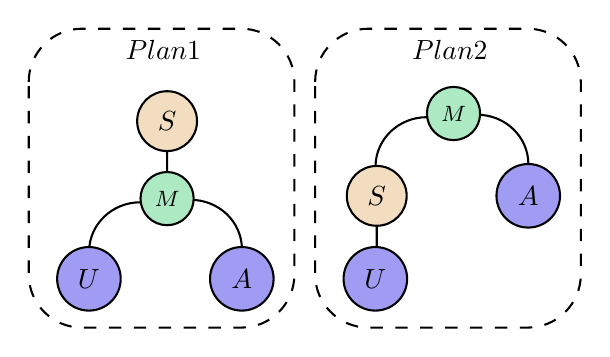
\begin{tikzpicture}[x=0.75pt,y=0.75pt,yscale=-1,xscale=1]
    %uncomment if require: \path (0,300); %set diagram left start at 0, and has height of 300
    
    %Rounded Rect [id:dp9327630093874044] 
    \draw  [dash pattern={on 4.5pt off 4.5pt}] (89,74.1) .. controls (89,59.96) and (100.46,48.5) .. (114.6,48.5) -- (191.4,48.5) .. controls (205.54,48.5) and (217,59.96) .. (217,74.1) -- (217,166.9) .. controls (217,181.04) and (205.54,192.5) .. (191.4,192.5) -- (114.6,192.5) .. controls (100.46,192.5) and (89,181.04) .. (89,166.9) -- cycle ;
    %Shape: Arc [id:dp8672386781469543] 
    \draw  [draw opacity=0] (118.09,155.74) .. controls (118.2,142.68) and (129.23,132.12) .. (142.82,132.12) -- (142.82,155.94) -- cycle ; \draw   (118.09,155.74) .. controls (118.2,142.68) and (129.23,132.12) .. (142.82,132.12) ;  
    %Shape: Arc [id:dp7960733152026014] 
    \draw  [draw opacity=0] (167,130.94) .. controls (180.66,130.94) and (191.73,141.6) .. (191.73,154.76) -- (167,154.76) -- cycle ; \draw   (167,130.94) .. controls (180.66,130.94) and (191.73,141.6) .. (191.73,154.76) ;  
    %Straight Lines [id:da6364636081987307] 
    \draw    (155.68,120.48) -- (155.67,107.08) ;
    
    
    %Rounded Rect [id:dp3039201957845239] 
    \draw  [dash pattern={on 4.5pt off 4.5pt}] (227,74.1) .. controls (227,59.96) and (238.46,48.5) .. (252.6,48.5) -- (329.4,48.5) .. controls (343.54,48.5) and (355,59.96) .. (355,74.1) -- (355,166.9) .. controls (355,181.04) and (343.54,192.5) .. (329.4,192.5) -- (252.6,192.5) .. controls (238.46,192.5) and (227,181.04) .. (227,166.9) -- cycle ;
    %Shape: Arc [id:dp6442642109452921] 
    \draw  [draw opacity=0] (256.09,114.74) .. controls (256.2,101.68) and (267.23,91.12) .. (280.82,91.12) -- (280.82,114.94) -- cycle ; \draw   (256.09,114.74) .. controls (256.2,101.68) and (267.23,91.12) .. (280.82,91.12) ;  
    %Shape: Arc [id:dp9997590238443537] 
    \draw  [draw opacity=0] (305,89.94) .. controls (305,89.94) and (305,89.94) .. (305,89.94) .. controls (318.66,89.94) and (329.73,100.6) .. (329.73,113.76) -- (305,113.76) -- cycle ; \draw   (305,89.94) .. controls (305,89.94) and (305,89.94) .. (305,89.94) .. controls (318.66,89.94) and (329.73,100.6) .. (329.73,113.76) ;  
    
    %Straight Lines [id:da7145621913901639] 
    \draw    (256.68,156.48) -- (256.67,143.08) ;

    % Text Node
    \draw  [fill={rgb, 255:red, 242; green, 221; blue, 192 }  ,fill opacity=1 ]  (155.67, 93.03) circle [x radius= 14.42, y radius= 14.42]   ;
    \draw (155.67,93.03) node    {$\text{S}$};
    % Text Node
    \draw  [fill={rgb, 255:red, 173; green, 234; blue, 195 }  ,fill opacity=1 ]  (155.67, 130.36) circle [x radius= 12.81, y radius= 12.81]   ;
    \draw (155.67,130.36) node  [font=\footnotesize]  {$\text{M}$};
    % Text Node
    \draw  [fill={rgb, 255:red, 160; green, 156; blue, 243 }  ,fill opacity=1 ]  (118.01, 169) circle [x radius= 15.31, y radius= 15.31]   ;
    \draw (118.01,169) node   [align=left] {$\displaystyle U$};
    % Text Node
    \draw  [fill={rgb, 255:red, 160; green, 156; blue, 243 }  ,fill opacity=1 ]  (191.67, 169) circle [x radius= 15.31, y radius= 15.31]   ;
    \draw (191.67,169) node   [align=left] {$\displaystyle A$};
    % Text Node
    \draw (134.17,52.73) node [anchor=north west][inner sep=0.75pt]    {$\text{Plan 1}$};
    % Text Node
    \draw  [fill={rgb, 255:red, 242; green, 221; blue, 192 }  ,fill opacity=1 ]  (256.67, 129.03) circle [x radius= 14.42, y radius= 14.42]   ;
    \draw (256.67,129.03) node    {$\text{S}$};
    % Text Node
    \draw  [fill={rgb, 255:red, 173; green, 234; blue, 195 }  ,fill opacity=1 ]  (293.67, 89.36) circle [x radius= 12.81, y radius= 12.81]   ;
    \draw (293.67,89.36) node  [font=\footnotesize]  {$\text{M}$};
    % Text Node
    \draw (272.17,52.73) node [anchor=north west][inner sep=0.75pt]    {$\text{Plan 2}$};
    % Text Node
    \draw  [fill={rgb, 255:red, 160; green, 156; blue, 243 }  ,fill opacity=1 ]  (256.01, 169) circle [x radius= 15.31, y radius= 15.31]   ;
    \draw (256.01,169) node   [align=left] {$\displaystyle U$};
    % Text Node
    \draw  [fill={rgb, 255:red, 160; green, 156; blue, 243 }  ,fill opacity=1 ]  (329.67, 129) circle [x radius= 15.31, y radius= 15.31]   ;
    \draw (329.67,129) node   [align=left] {$\displaystyle A$};
    
    
    \end{tikzpicture}
    \caption{Two example query plans for the sql query from figure \ref{figure:sql_query_example}.}
    \label{figure:example_query_plans}
\end{figure}

\newpage


In a large system that handles multiple requests per second, plans from different queries can have operations that are shared across. Combining these sub-sequences together can save additional execution time\cite{roy_multi-query_2009}. Finding the best combination of multiple queries and their plans has been proven to be an \emph{NP-Hard} problem\cite{sellis_multiple-query_1990}. This can be done classically with an exhaustive algorithm in $O(P^Q)$\footnote{as long as all queries have the same number of plans}, where $P$ is the number of plans and $Q$ the number of queries, as shown in listing \ref{figure:pseudocode_bruteforce_search}. The work of Kathurina et al.\cite{kathuria_provable_mqo} offers a greedy algorithm for finding a \emph{good} solution, whilst also proving that finding a better approximation factor for the greedy algorithm is \emph{NP-Hard}. A hybrid approach that combines classical and quantum computing uses QAOA (short for Quantum Approximate Optimization Algorithm)\cite{farhi_quantum_2014} has been shown to be quasi-optimal solution finders with a runtime of $O(I \cdot (PQ)^2)$\cite{fankhauser_multiple_2021}. \par


\begin{listing}[!ht]
    \centering
    \begin{minted}{python}
        for plan_a in plans:
            for plan_b in plans:
                if plan_a.query != plan_b.query:
                    if savings(plan_a, plan_b) > current_savings:
                        current_savings = savings(plan_a, plan_b)
                        cheapest_combination = <plan_a, plan_b>
    \end{minted}
    \caption{Pseudocode of an exhaustive algorithm that tries every possible combination and finds the cheapest one.}
    \label{figure:pseudocode_bruteforce_search}
\end{listing}

 For example, if a second query that also filters the table $U$ for \code{USERS.NAME = "Abraham"} is supposed to run at roughly the same time, they could share a portion of the task. As shown in figure \ref{figure:example_query_plans}, the plans consist of multiple different instructions. Each instruction in any plan consist of single operations applied to tables of the database that are based on relational algebra\cite{codd_relational_1970}\footnote{But not limited to them, as modern databases also include hashing and indexing in the plans. Nonetheless, these operations can also be combined to save previous runtime}. 
 
 \newpage
 
 Figure \ref{figure:plan_tree} shows how the plans $\mathcal{Q}_0\mathcal{P}_0$ and $\mathcal{Q}_1\mathcal{P}_0$, from the differing queries $\mathcal{Q}_0$ and $\mathcal{Q}_1$, contain parts that can be reused, as shown in figure \ref{figure:plan_tree}. 

\begin{figure}[!h]
    \centering
\tikzset{every picture/.style={line width=0.75pt}} %set default line width to 0.75pt        

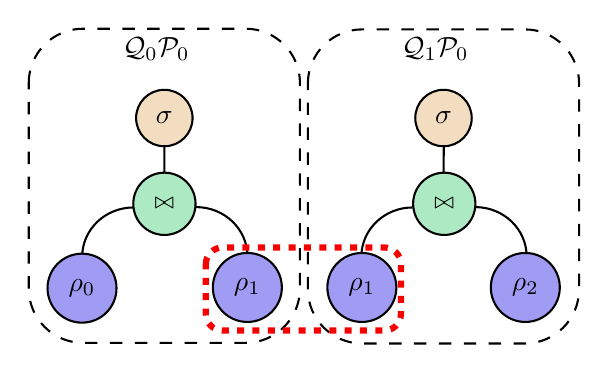
\begin{tikzpicture}[x=0.75pt,y=0.75pt,yscale=-1,xscale=1]
%uncomment if require: \path (0,300); %set diagram left start at 0, and has height of 300

%Rounded Rect [id:dp3098689700784747] 
\draw  [dash pattern={on 4.5pt off 4.5pt}] (120.33,155.05) .. controls (120.33,140.62) and (132.03,128.92) .. (146.47,128.92) -- (224.87,128.92) .. controls (239.3,128.92) and (251,140.62) .. (251,155.05) -- (251,254.12) .. controls (251,268.55) and (239.3,280.25) .. (224.87,280.25) -- (146.47,280.25) .. controls (132.03,280.25) and (120.33,268.55) .. (120.33,254.12) -- cycle ;
%Shape: Arc [id:dp8469571253916317] 
\draw  [draw opacity=0] (146.09,238.65) .. controls (146.2,225.59) and (157.23,215.04) .. (170.82,215.04) -- (170.82,238.86) -- cycle ; \draw   (146.09,238.65) .. controls (146.2,225.59) and (157.23,215.04) .. (170.82,215.04) ;  
%Shape: Arc [id:dp8173590455021038] 
\draw  [draw opacity=0] (201,214.86) .. controls (214.66,214.86) and (225.73,225.52) .. (225.73,238.67) -- (201,238.67) -- cycle ; \draw   (201,214.86) .. controls (214.66,214.86) and (225.73,225.52) .. (225.73,238.67) ;  
%Straight Lines [id:da6630213040029864] 
\draw    (185.68,199.4) -- (185.67,186) ;
%Rounded Rect [id:dp5436966787626745] 
\draw  [dash pattern={on 4.5pt off 4.5pt}] (254.83,155.38) .. controls (254.83,140.95) and (266.53,129.25) .. (280.97,129.25) -- (359.37,129.25) .. controls (373.8,129.25) and (385.5,140.95) .. (385.5,155.38) -- (385.5,254.45) .. controls (385.5,268.88) and (373.8,280.58) .. (359.37,280.58) -- (280.97,280.58) .. controls (266.53,280.58) and (254.83,268.88) .. (254.83,254.45) -- cycle ;
%Shape: Arc [id:dp13654717695684715] 
\draw  [draw opacity=0] (280.59,238.65) .. controls (280.7,225.59) and (291.73,215.04) .. (305.32,215.04) -- (305.32,238.86) -- cycle ; \draw   (280.59,238.65) .. controls (280.7,225.59) and (291.73,215.04) .. (305.32,215.04) ;  
%Shape: Arc [id:dp7676498647138272] 
\draw  [draw opacity=0] (335.5,214.86) .. controls (349.16,214.86) and (360.23,225.52) .. (360.23,238.67) -- (335.5,238.67) -- cycle ; \draw   (335.5,214.86) .. controls (349.16,214.86) and (360.23,225.52) .. (360.23,238.67) ;  
%Straight Lines [id:da7192788563309687] 
\draw    (320.18,199.4) -- (320.33,184.44) ;
%Rounded Rect [id:dp6770297453454031] 
\draw  [color={rgb, 255:red, 246; green, 1; blue, 1 }  ,draw opacity=1 ][dash pattern={on 2.53pt off 3.02pt}][line width=2.25]  (205.67,242.33) .. controls (205.67,237.92) and (209.25,234.33) .. (213.67,234.33) -- (291.67,234.33) .. controls (296.08,234.33) and (299.67,237.92) .. (299.67,242.33) -- (299.67,266.33) .. controls (299.67,270.75) and (296.08,274.33) .. (291.67,274.33) -- (213.67,274.33) .. controls (209.25,274.33) and (205.67,270.75) .. (205.67,266.33) -- cycle ;

% Text Node
\draw (164.17,131.65) node [anchor=north west][inner sep=0.75pt]    {$\mathcal{Q}_{0}\mathcal{P}_{0}$};
% Text Node
\draw  [fill={rgb, 255:red, 242; green, 221; blue, 192 }  ,fill opacity=1 ]  (185.67, 171.95) circle [x radius= 13.6, y radius= 13.6]   ;
\draw (185.67,171.95) node    {$\sigma $};
% Text Node
\draw (298.67,131.65) node [anchor=north west][inner sep=0.75pt]    {$\mathcal{Q}_{1}\mathcal{P}_{0}$};
% Text Node
\draw  [fill={rgb, 255:red, 242; green, 221; blue, 192 }  ,fill opacity=1 ]  (320.17, 171.95) circle [x radius= 13.6, y radius= 13.6]   ;
\draw (320.17,171.95) node    {$\sigma $};
% Text Node
\draw  [fill={rgb, 255:red, 173; green, 234; blue, 195 }  ,fill opacity=1 ]  (185.71, 213.28) circle [x radius= 15, y radius= 15]   ;
\draw (185.71,213.28) node  [font=\footnotesize]  {$\bowtie $};
% Text Node
\draw  [fill={rgb, 255:red, 173; green, 234; blue, 195 }  ,fill opacity=1 ]  (320.54, 213.28) circle [x radius= 15, y radius= 15]   ;
\draw (320.54,213.28) node  [font=\footnotesize]  {$\bowtie $};
% Text Node
\draw  [fill={rgb, 255:red, 160; green, 156; blue, 243 }  ,fill opacity=1 ]  (146.01, 253.92) circle [x radius= 16.62, y radius= 16.62]   ;
\draw (146.01,253.92) node   [align=left] {$\displaystyle \rho _{0}$};
% Text Node
\draw  [fill={rgb, 255:red, 160; green, 156; blue, 243 }  ,fill opacity=1 ]  (225.67, 253.58) circle [x radius= 16.62, y radius= 16.62]   ;
\draw (225.67,253.58) node   [align=left] {$\displaystyle \rho _{1}$};
% Text Node
\draw  [fill={rgb, 255:red, 160; green, 156; blue, 243 }  ,fill opacity=1 ]  (280.84, 253.58) circle [x radius= 16.62, y radius= 16.62]   ;
\draw (280.84,253.58) node   [align=left] {$\displaystyle \rho _{1}$};
% Text Node
\draw  [fill={rgb, 255:red, 160; green, 156; blue, 243 }  ,fill opacity=1 ]  (359.59, 253.58) circle [x radius= 16.62, y radius= 16.62]   ;
\draw (359.59,253.58) node   [align=left] {$\displaystyle \rho _{2}$};


\end{tikzpicture}


    \caption{Two differing plans $\mathcal{Q}_0\mathcal{P}_0$ and $\mathcal{Q}_1\mathcal{P}_1$, which serve different goals but contain the same operation $\rho_1$, marked in the red dotted box}
    \label{figure:plan_tree}
\end{figure}

Plans, costs, and savings can be mathematically expressed. Let there be given function $\mathcal{C}$ which returns the cost for a given operation or collection of operations, as defined in equation \ref{equation:formal_cost_function}. Let there also be a given function $\mathcal{S}$, which calculates the savings two collections of operations can achieve, as shown in equation \ref{equation:formal_savings_function}.

\begin{equation}
    \centering
    \begin{split}
        \mathcal{C}(\mathcal{Q}_0\mathcal{P}_1) =\ 45 \\
        \mathcal{C}(\rho_1) =\ 15 \\
    \end{split}
    \label{equation:formal_cost_function}
\end{equation}

\begin{equation}
    \centering
    \begin{split}
        \mathcal{S}(\mathcal{Q}_0\mathcal{P}_1, \mathcal{Q}_1\mathcal{P}_0) =\ 15 \\
        \mathcal{S}(\mathcal{Q}_0\mathcal{P}_0, \mathcal{Q}_1\mathcal{P}_1) =\ 0 \\
    \end{split}
    \label{equation:formal_savings_function}
\end{equation}


Taking a problem consisting of two queries $\mathcal{Q}_0$ and $\mathcal{Q}_1$, each of which has two plans $\mathcal{P}_0$ and $\mathcal{P}_1$, we can calculate the total costs of running them collectively as shown in equation \ref{equation:formal_total_cost_calculation}.

\begin{equation}
    \centering
    \begin{split}
        \mathcal{C}(\mathcal{Q}_0\mathcal{P}_0) + \mathcal{C}(\mathcal{Q}_1\mathcal{P}_0) - \mathcal{S}(\mathcal{Q}_0\mathcal{P}_0, \mathcal{Q}_1\mathcal{P}_0) \\
        \mathcal{C}(\mathcal{Q}_0\mathcal{P}_0) + \mathcal{C}(\mathcal{Q}_1\mathcal{P}_1) - \mathcal{S}(\mathcal{Q}_0\mathcal{P}_0, \mathcal{Q}_1\mathcal{P}_1) \\
        \mathcal{C}(\mathcal{Q}_0\mathcal{P}_1) + \mathcal{C}(\mathcal{Q}_1\mathcal{P}_0) - \mathcal{S}(\mathcal{Q}_0\mathcal{P}_1, \mathcal{Q}_1\mathcal{P}_0) \\
        \mathcal{C}(\mathcal{Q}_0\mathcal{P}_1) + \mathcal{C}(\mathcal{Q}_1\mathcal{P}_1) - \mathcal{S}(\mathcal{Q}_0\mathcal{P}_1, \mathcal{Q}_1\mathcal{P}_1) \\
    \end{split}
    \label{equation:formal_total_cost_calculation}
\end{equation}

If we change the problem space from two queries to more, or create a differing number of plans per query, the given complexity changes.

